% -*- coding: utf-8 -*-
%-------------------------designed by zcf--------------
\documentclass[UTF8,a4paper,10pt]{ctexart}
\usepackage[left=3.17cm, right=3.17cm, top=2.74cm, bottom=2.74cm]{geometry}
\usepackage{amsmath}
\usepackage{graphicx,subfig}
\usepackage{float}
\usepackage{cite}
\usepackage{caption}
\usepackage{enumerate}
\usepackage{booktabs} %表格
\usepackage{multirow}
\newcommand{\tabincell}[2]{\begin{tabular}{@{}#1@{}}#2\end{tabular}}  %表格强制换行
%-------------------------字体设置--------------
\usepackage{times} 
\newcommand{\yihao}{\fontsize{26pt}{36pt}\selectfont}           % 一号, 1.4 倍行距
\newcommand{\erhao}{\fontsize{22pt}{28pt}\selectfont}          % 二号, 1.25倍行距
\newcommand{\xiaoer}{\fontsize{18pt}{18pt}\selectfont}          % 小二, 单倍行距
\newcommand{\sanhao}{\fontsize{16pt}{24pt}\selectfont}  %三号字
\newcommand{\xiaosan}{\fontsize{15pt}{22pt}\selectfont}        % 小三, 1.5倍行距
\newcommand{\sihao}{\fontsize{14pt}{21pt}\selectfont}            % 四号, 1.5 倍行距
\newcommand{\banxiaosi}{\fontsize{13pt}{19.5pt}\selectfont}    % 半小四, 1.5倍行距
\newcommand{\xiaosi}{\fontsize{12pt}{18pt}\selectfont}            % 小四, 1.5倍行距
\newcommand{\dawuhao}{\fontsize{11pt}{11pt}\selectfont}       % 大五号, 单倍行距
\newcommand{\wuhao}{\fontsize{10.5pt}{15.75pt}\selectfont}    % 五号, 单倍行距
%-------------------------章节名----------------
\usepackage{ctexcap} 
\CTEXsetup[name={,、},number={ \chinese{section}}]{section}
\CTEXsetup[name={(,)},number={\chinese{subsection}}]{subsection}
\CTEXsetup[name={,.},number={\arabic{subsubsection}}]{subsubsection}
%-------------------------页眉页脚--------------
\usepackage{fancyhdr}
\pagestyle{fancy}
\lhead{\kaishu \leftmark}
% \chead{}
\rhead{\kaishu 计算机系统设计作业报告}%加粗\bfseries 
\lfoot{}
\cfoot{\thepage}
\rfoot{}
\renewcommand{\headrulewidth}{0.1pt}  
\renewcommand{\footrulewidth}{0pt}%去掉横线
\newcommand{\HRule}{\rule{\linewidth}{0.5mm}}%标题横线
\newcommand{\HRulegrossa}{\rule{\linewidth}{1.2mm}}
%-----------------------伪代码------------------
\usepackage{algorithm}  
\usepackage{algorithmicx}  
\usepackage{algpseudocode}  
\floatname{algorithm}{Algorithm}  
\renewcommand{\algorithmicrequire}{\textbf{Input:}}  
\renewcommand{\algorithmicensure}{\textbf{Output:}} 
\usepackage{lipsum}  
\makeatletter
\newenvironment{breakablealgorithm}
  {% \begin{breakablealgorithm}
  \begin{center}
     \refstepcounter{algorithm}% New algorithm
     \hrule height.8pt depth0pt \kern2pt% \@fs@pre for \@fs@ruled
     \renewcommand{\caption}[2][\relax]{% Make a new \caption
      {\raggedright\textbf{\ALG@name~\thealgorithm} ##2\par}%
      \ifx\relax##1\relax % #1 is \relax
         \addcontentsline{loa}{algorithm}{\protect\numberline{\thealgorithm}##2}%
      \else % #1 is not \relax
         \addcontentsline{loa}{algorithm}{\protect\numberline{\thealgorithm}##1}%
      \fi
      \kern2pt\hrule\kern2pt
     }
  }{% \end{breakablealgorithm}
     \kern2pt\hrule\relax% \@fs@post for \@fs@ruled
  \end{center}
  }
\makeatother
%------------------------代码-------------------
\usepackage{xcolor} 
\usepackage{listings} 
\usepackage{fontspec}
\newfontfamily\menlo{Menlo}
\setmonofont[Mapping={}]{Monaco} 
\definecolor{mygreen}{rgb}{0,0.6,0}
\definecolor{mygray}{rgb}{0.5,0.5,0.5}
\definecolor{mymauve}{rgb}{0.58,0,0.82}
\lstset{ %
backgroundcolor=\color{white},   % choose the background color
basicstyle=\footnotesize\ttfamily,        % size of fonts used for the code
columns=fullflexible,
breaklines=true,                 % automatic line breaking only at whitespace
captionpos=b,                    % sets the caption-position to bottom
tabsize=4,
commentstyle=\color{mygreen},    % comment style
escapeinside={\%*}{*)},          % if you want to add LaTeX within your code
keywordstyle=\color{blue},       % keyword style
stringstyle=\color{mymauve}\ttfamily,     % string literal style
frame=single,
rulesepcolor=\color{red!20!green!20!blue!20},
numbers=left,
 numberstyle=\tiny\menlo
% identifierstyle=\color{red},
% language=c++,
}
%------------超链接----------
\usepackage[colorlinks,linkcolor=black,anchorcolor=blue]{hyperref}
%------------------------TODO-------------------
\usepackage{enumitem,amssymb}
\newlist{todolist}{itemize}{2}
\setlist[todolist]{label=$\square$}
% for check symbol 
\usepackage{pifont}
\newcommand{\cmark}{\ding{51}}%
\newcommand{\xmark}{\ding{55}}%
\newcommand{\done}{\rlap{$\square$}{\raisebox{2pt}{\large\hspace{1pt}\cmark}}\hspace{-2.5pt}}
\newcommand{\wontfix}{\rlap{$\square$}{\large\hspace{1pt}\xmark}}
%------------------------水印-------------------
\usepackage{tikz}
\usepackage{xcolor}
\usepackage{eso-pic}

\newcommand{\watermark}[3]{\AddToShipoutPictureBG{
\parbox[b][\paperheight]{\paperwidth}{
\vfill%
\centering%
\tikz[remember picture, overlay]%
  \node [rotate = #1, scale = #2] at (current page.center)%
    {\textcolor{gray!80!cyan!30!magenta!30}{#3}};
\vfill}}}



%———————————————————————————————————————————正文———————————————————————————————————————————————
%----------------------------------------------
\begin{document}
\begin{titlepage}
    \begin{center}
    
\includegraphics[width=0.8\textwidth]{NKU.png}\\[1cm]    
    \textsc{\Huge \kaishu{\textbf{南\ \ \ \ \ \ 开\ \ \ \ \ \ 大\ \ \ \ \ \ 学}} }\\[0.9cm]
    \textsc{\huge \kaishu{\textbf{计\ \ 算\ \ 机\ \ 学\ \ 院}}}\\[0.5cm]
    \textsc{\Large \textbf{计算机系统设计作业报告}}\\[0.8cm]
    \HRule \\[0.9cm]
    { \LARGE \bfseries PA实验一报告}\\[0.4cm]
    \HRule \\[2.0cm]
    \centering
    \textsc{\LARGE \kaishu{朱浩泽\ 1911530}}\\[0.5cm]
    \textsc{\LARGE \kaishu{年级\ :\ 2019级}}\\[0.5cm]
    \textsc{\LARGE \kaishu{专业\ :\ 计算机科学与技术}}\\[0.5cm]
    \textsc{\LARGE \kaishu{指导教师\ :\ 卢冶}}\\[0.5cm]
    \vfill
    {\Large \today}
    \end{center}
\end{titlepage}
% -------------摘------要--------------
\newpage
% \thispagestyle{empty}
% \renewcommand{\abstractname}{\kaishu \sihao \textbf{摘要}}
%     \begin{abstract}

%         \noindent  %顶格
%         \textbf{\\\ 关键字:Parallel}\textbf{} \\\ \\\
%     \end{abstract}
% % ----------------------------------------------------------------
\tableofcontents
% ----------------------------------------------------------------
\newpage
\watermark{60}{10}{NKU}
\setcounter{page}{1}
\section{概述}
%——————————————————————————————————————
\subsection{实验目的}
熟悉基础设施的各种工具和手段;熟悉寄存器间的存储关系;学习实现简易调试器
补充指令;学习表达式求值,监视点的实现方法
\subsection{实验内容}
\begin{itemize}
  \item \textbf{阶段一}
  \begin{itemize}
    \item [$\circ $] 实现正确的寄存器结构体
    \item [$\circ $] 实现解析命令
    \item [$\circ $] 实现单步执行
    \item [$\circ $] 实现打印寄存器
    \item [$\circ $] 实现内存扫描
  \end{itemize}
  \item \textbf{阶段二}
  \begin{itemize}
    \item [$\circ $] 实现表达式求值
    \item [$\circ $] 实现词法分析
    \item [$\circ $] 实现递归求值
    \item [$\circ $] 实现调试中的表达式求值
  \end{itemize}
  \item \textbf{阶段三}
  \begin{itemize}
    \item [$\circ $] 实现断点
    \item [$\circ $] 实现监视点
  \end{itemize}
\end{itemize}
%——————————————————————————————————————
\section{阶段一}
\subsection{实现正确的寄存器结构体}
\begin{itemize}
  \item 为了实现32位、16位、8位寄存器各8个和一个程序计数器eip,我们利用匿名Union各个变量互斥并共享同一内存首地址这一特点,来实现这一结构体
  \item 修改nemu/include/cpu/reg.h中的代码如下
  \begin{lstlisting}[language = C]    
typedef struct {
  union{
    /* data */
    union {
      uint32_t _32;
      uint16_t _16;
      uint8_t _8[2];
    } gpr[8];
    struct 
    {
      rtlreg_t eax, ecx, edx, ebx, esp, ebp, esi, edi;
    };
  };
  vaddr_t eip;
} CPU_state;
  \end{lstlisting}
  \item 在上面的代码中,grp中的的\_32代表的是eax中的32位,\_16代表的是ax中的16位,\_8[2]分别代表的是ah中的8到16位和al中的0到8位
\end{itemize}
\subsection{实现解析命令}
\begin{itemize}
  \item 在nemu/src/monitor/debug/ui.c中实现命令表,其代码如下
  \begin{lstlisting}[language = C]
static struct {
  char *name;
  char *description;
  int (*handler) (char *);
} cmd_table [] = {
  { "help", "Display informations about all supported commands", cmd_help },
  { "c", "Continue the execution of the program", cmd_c },
  { "q", "Exit NEMU", cmd_q },

  /* TODO: Add more commands */

  { "si", "args:[N]; exectue [N] instructions step by step", cmd_si}, //让程序单步执行 N 条指令后暂停执行, 当N没有给出时, 缺省为1
  { "info", "args:r/w;print information about register or watch point ", cmd_info}, //打印寄存器状态
  { "x", "x [N] [EXPR];sacn the memory", cmd_x }, //内存扫描
  { "p", "expr", cmd_p}, //表达式
  { "w", "set the watchpoint", cmd_w}, //添加监视点
  { "d", "delete the watchpoint", cmd_d} //删除监视点
};
  \end{lstlisting}
  \item 其执行效果如下图所示
  \begin{center}
    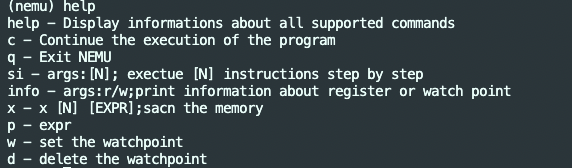
\includegraphics[scale = 0.6]{4}
  \end{center}
  
\end{itemize}
\subsection{实现单步执行}
\begin{itemize}
  \item  在nemu/src/monitor/debug/ui.c添加cmd\_si函数,其代码如下
  \begin{lstlisting}[language = C]
static int cmd_si(char *args) {
  uint64_t N = 0;
  if(args == NULL) {
    N = 1;
  }
  else {
    int temp = sscanf(args, "%lu", &N);
    if(temp <= 0) {
      printf("args error in cmd_si\n");
      return 0;
    }
  }
  cpu_exec(N);
  return 0;
}
  \end{lstlisting}
  \item 执行效果如下图所示,输入si和要执行的步骤N,进行打印
  \begin{center}
    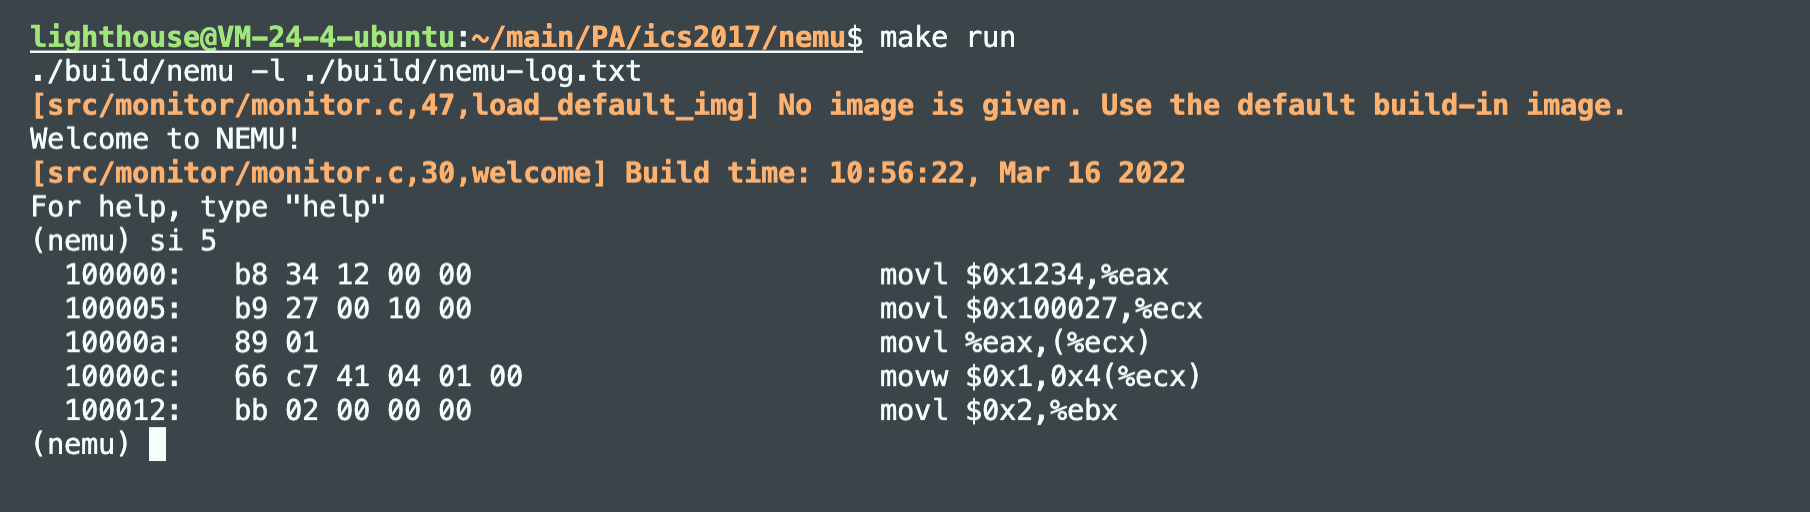
\includegraphics[scale = 0.43]{5}
  \end{center}
\end{itemize}
\subsection{实现打印寄存器}
\begin{itemize}
  \item 在nemu/src/monitor/debug/ui.c添加cmd\_info函数,其代码如下,输入参数r对寄存器直接进行打印,输入参数w对监视点进行打印
  \begin{lstlisting}[language = c++]
static int cmd_info(char *args) {
  char s;
  if(args == NULL) {
    printf("args error in cmd_info (miss args)\n");
    return 0;
  }
  int temp = sscanf(args, "%c", &s);
  if(temp <= 0) {
    //解析失败
    printf("args error in cmd_info\n");
    return 0;
  }
  if(s == 'w') {
    //打印监视点信息
    print_wp();;
    return 0;
  }
  if(s == 'r') {
    //打印寄存器
    //32bit
    for(int i = 0; i < 8; i++) {
      printf("%s  0x%x\n", regsl[i], reg_l(i));
    }
    printf("eip  0x%x\n", cpu.eip);
    //16bit
    for(int i = 0; i < 8; i++) {
      printf("%s  0x%x\n", regsw[i], reg_w(i));
    }
    //8bit
    for(int i = 0; i < 8; i++)
    {
      printf("%s  0x%x\n", regsb[i], reg_b(i));
    }
    return 0;
  }
  //如果产生错误
  printf("args error in cmd_info\n");
  return 0;
}
  \end{lstlisting}
  \item 执行效果如下图所示
  \begin{center}
    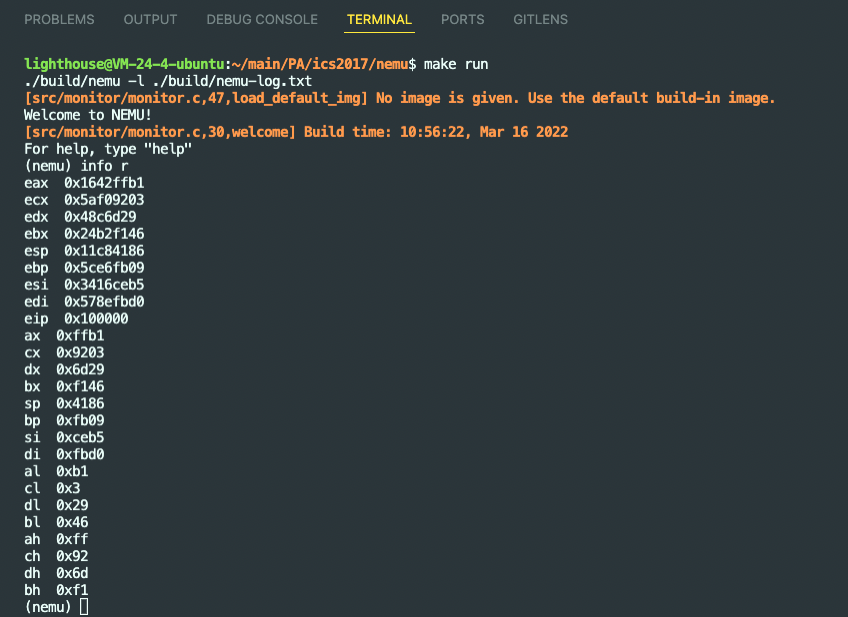
\includegraphics[scale = 0.4]{2}
  \end{center}
\end{itemize}
\subsection{实现内存扫描}
\begin{itemize}
  \item 在nemu/src/monitor/debug/ui.c添加cmd\_x函数,其代码如下
  \begin{lstlisting}[language = C]
static int cmd_x(char *args) {
  int nLen = 0;
  vaddr_t addr;
  int temp = sscanf(args, "%d 0x%x", &nLen, &addr);
  if(temp <= 0) {
    //解析失败
    printf("args error in cmd_si\n");
    return 0;
  }
  printf("Memory:");
  for(int i = 0; i < nLen; i++) {
    if(i % 4 == 0) {
      printf("\n0x%x:  0x%02x", addr + i, vaddr_read(addr + i, 1));
    }  
    else {
      printf("  0x%02x", vaddr_read(addr + i, 1));
    }
  }
  printf("\n");
  return 0;
}
  \end{lstlisting}
  \item 该函数主要是调用了nemu/src/memory/memory.c中的vaddr\_read函数进行内存扫描
  \item 执行效果如下图所示
  \begin{center}
    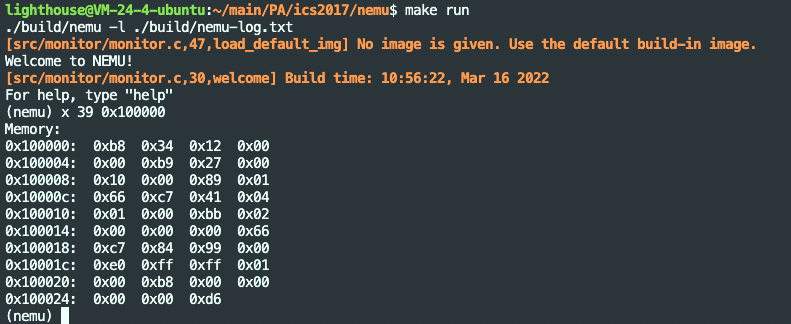
\includegraphics[scale = 0.45]{3}
  \end{center}
\end{itemize}

\section{阶段二}
\subsection{表达式求值的计算}
在有了编译原理课程的基础后,我们可以知道,表达式求值的过程是先将整个句子切分为各个token,然后对各个token按照赋予的优先级进行分割后求返回值,最终通过这种递归运算求出整个表达式的值。
\par 在这个求值过程中,我们需要注意寄存器的值是可以当作操作数进行运算的,且对于括号的操作跟编译原理中直接利用lex工具


\section{}
\subsection{第一节}
如图\ref{fig:1}所示
\begin{figure}[H]
    \centering
    
\includegraphics[scale=0.3]{NKU.png}
    \caption{Caption}
    \label{fig:1}
\end{figure}

表
\begin{table}[!htbp]
  \centering
  \begin{tabular}{ccccccccccc}
  \toprule  
  N/n$\backslash$Algo& naive-conv& naive-pool& omp-conv& omp-pool\\
  \midrule
  64/2& 0.0167& 0.01255& 0.04142& 0.03799\\
  64/4& 0.03599&0.0394& 0.0458& 0.0421\\
  \bottomrule
  \end{tabular}
  \caption{性能测试结果(4线程)(单位:ms)}
\end{table}

带单元格表格
\begin{table}[!htbp]
  \centering
  \begin{tabular}{|c|c|c|c|c|c|c|}
  \hline
  \multicolumn{2}{|c|}{ \multirow{2}*{$Cost$} }& \multicolumn{5}{c|}{To}\\
  \cline{3-7}
  \multicolumn{2}{|c|}{}&$A$&$B$&$C$&$D$&$E$\\
  \hline
  \multirow{3}*{From}&$B$&7&0&1&3&8\\
  \cline{2-7}
  &$C$&8&1&0&2&7\\
  \cline{2-7}
  &$D$&8&3&2&0&5\\
  \hline
  \end{tabular}
  \caption{结点C距离向量表(无毒性逆转)}
\end{table}

%——————————————————————————————————————
\subsection{第二节}
伪代码

\begin{breakablealgorithm} 
  \caption{初始化obj文件信息——对应MeshSimplify类中readfile函数,Face类calMatrix函数} 
  \begin{algorithmic}[1] %每行显示行号  
      \Require obj文件,顶点、边、面列表
      \Ensure 是否读取成功
      \Function {calMatrix}{$Face$}  
              \State $normal \gets e1×e2$  
              \State $normal \gets normal/normal.length$
              \State $temp[] \gets {normal.x, normal.y, normal.z, normal· Face.v1}$
              \State $Matrix[i][j]=temp[i] * temp[j]$ 
              \State \Return{$Matrix$}  
      \EndFunction
      \State 根据obj的v和f区分点面信息,读取并加入列表
      \State $scale \gets $记录点坐标中距离原点最远的分量,以便后续OpenGL进行显示
      \State $ori \gets $记录中心点,便于OpenGL显示在中心位置,避免有的obj偏移原点较多
      \State 根据三角面片信息,计算一个面的三条边
      \State 计算每个面的矩阵$\gets calMatrix$
      \State 将每个面的矩阵加到各点,由点维护\\
      \Return True
  \end{algorithmic}  
\end{breakablealgorithm}

代码
\begin{lstlisting}[title=逐列访问平凡算法,frame=trbl,language={C++}]
  void ord()   
  {
      double head,tail,freq,head1,tail1,timess=0; // timers
      init(N);
      QueryPerformanceFrequency((LARGE_INTEGER *)&freq );
      QueryPerformanceCounter((LARGE_INTEGER *)&head);
      for (int i=0; i<NN; i++)
          for (int j=0; j<NN; j++)
              col_sum[i] += (b[j][i]*a[j]);
      QueryPerformanceCounter ((LARGE_INTEGER *)& tail) ;
      cout << "\nordCol" <<(tail-head)*1000.0 / freq<< "ms" << endl;
  }
\end{lstlisting}


%——————————————————————————————————————
\subsection{第三节}

参考文献\cite{adams1995hitchhiker}\cite{shin2016deep}
    
多行公式
\begin{align}
  a+b = a + b \\
  \frac{a+b}{a-b}
\end{align}

行内公式:$\sum^N_{i=1}$

\textbf{超链接}  \href{http://youtube.com/}{YouTube}

带标号枚举
\begin{enumerate}
  \item 1
  \item 2
\end{enumerate}

不带标号枚举
\begin{itemize}
  \item 1
  \item 2
\end{itemize}

\xiaosi{切换字体大小}

%----------------------------------------------------------------
\section{总结}

%----------------------------------------------------------------
\newpage
\bibliographystyle{plain}
\bibliography{references} 
\end{document}
